%課題研究レジュメテンプレート ver. 1.2

\documentclass[uplatex]{jsarticle}
\usepackage[top=20mm,bottom=20mm,left=20mm,right=20mm]{geometry}
\usepackage[T1]{fontenc}
\usepackage{txfonts}
\usepackage{wrapfig}
\usepackage[expert,deluxe]{otf}
\usepackage[dvipdfmx,hiresbb]{graphicx}
\usepackage[dvipdfmx]{hyperref}
\usepackage{pxjahyper}
\usepackage{secdot}

\makeatletter
  \renewcommand{\section}{%
    \if@slide\clearpage\fi
    \@startsection{section}{1}{\z@}%
    {\Cvs \@plus.5\Cdp \@minus.2\Cdp}% 前アキ
    {.5\Cvs \@plus.3\Cdp}% 後アキ
    %{\normalfont\Large\headfont\raggedright}}
    {\normalfont\raggedright}}

  \renewcommand{\subsection}{\@startsection{subsection}{2}{\z@}%
    {\Cvs \@plus.5\Cdp \@minus.2\Cdp}% 前アキ
    {.5\Cvs \@plus.3\Cdp}% 後アキ
    %{\normalfont\large\headfont}}
    {\normalfont}}

  \renewcommand{\subsubsection}{\@startsection{subsubsection}{3}{\z@}%
    {\Cvs \@plus.5\Cdp \@minus.2\Cdp}%
    {\z@}%
    %{\normalfont\normalsize\headfont}}
    {\normalfont}}
\makeatother
%ここから上を編集する必要はない.

\title{\vspace{-14mm}プロジェクト進行中にWEBサービスの障害が発生した場合の影響}
\author{PMコース 矢吹研究室 1442012 岩瀬翔}
\date{}%日付を入れる必要はない.
\pagestyle{empty}%ページ番号は振らない.
\begin{document}
\maketitle

\section{研究の背景}
複数のメンバが同時に開発を行うソフトウェア開発プロジェクトでは,有用なWEBサービスを使いながら行われることがある.例えば「GitHub」というバージョン管理システムを用いることで,ファイルの最新バージョンが分からなくなってしまうといったリスクを低減することができる.他にもチーム内でコミュニケーションを取るためのチャットツール「Slack」やユーザレビューなどを行うために使用される「Skype」,チームで作成したファイルを共有できる「Google Drive」などがある.これらのWEBサービスに障害が発生した場合,プロジェクトへの影響が懸念されるのではないかと考えた.

中でもGitHubは企業においてもオープンソースソフトウェアとしてソースコードを公開し,企業内では見つけることの難しかった問題などをより早く発見し修正できるなどの理由から利用されている\cite{01}.そのGitHubのサーバーが2016年1月28日にダウンし,インターネット上で話題になったというニュースを目にした.実際にGitHubのサーバーダウンについて,Twitterを用いて調べてみたところ「仕事にならない」「卒論が書けない」などといった反応が多く見られた\cite{02}.

以上のことからプロジェクト進行中にGitHubで障害が発生した場合,どのような影響が生じ,その対策のために何かできることはないのかと考え研究することとした.

\section{研究の目的}
本研究の目的は次の3点を目標とする.
\begin{itemize}
 \item プロジェクトで使用されるWEBサービスに障害が発生した場合どれほどの人に影響が及ぶか調べる.
 \item プロジェクトで使用されるWEBサービスに障害が発生した場合どのような影響が発生するか特定する.
 \item WEBサービスの障害発生に対するリスク対策案を考案する.
\end{itemize}
上記の目標を達成することを目的とし研究を行う.

\section{プロジェクトマネジメントとの関連}

本研究はプロジェクトマネジメントにおける10個の知識エリアのうち,リスクマネジメントに関連付けることができると考える.WEBサービスの障害はプロジェクトの進捗に関わる明確なリスクであるからだ.また,このリスク発生に対する事前対策を考案することができると考えたからでもある.

\section{研究の方法}
本研究は,プロジェクトで使用されている代表的なWEBサービスであるGitHubの障害発生時の状況について調査を行う.調査方法はTwitterを使用し,GitHubのサーバーダウンなど障害発生に関するツイートをデータとして収集する.データ収集の手順は以下の通りである\cite{03}.
\begin{enumerate}
 \item 「GitHub Status」を参照し,2016年で障害が発生したと記録されている時間を調べる.その時間近辺をTwitterで条件を指定し検索する(例:GitHub lang:ja since:2016-10-19 until:2016-10-21\_20:30:00\_JST).その後,必要な分だけブラウザをスクロールし,障害発生した旨のツイートから,復旧したという旨のツイートを表示する.ページ全体をローカルにHTMLファイルで保存する.
 \item HTMLファイルからツイートの時間と本文のみを抽出するため,Rubyを使ったクローラー開発を行う\cite{04}.
 \item 開発したクローラーを使用して保存済みのHTMLファイルからデータの抽出を行う.
 \item 以上の手順を障害発生時間ごとに繰り返す.
 \item 障害発生時の「GitHub」に対するツイート数,どのくらいの時間で復旧が完了するのかを調べる.
 \item 頻出単語の抽出を行い,どのような影響が発生しているのか,どのような反応があるのか分析する.
 \item 分析結果を基に,リスク対策案を考察する.
\end{enumerate}


\section{現在の進捗状況}
「GitHub Status」を参照して調べたところ,2016年のGitHubの障害発生回数は13回であった.クローラーを開発し,発生した障害それぞれについてデータの収集を完了した.そのデータから,13回分それぞれのツイート数と障害が発生していた時間で2つのグラフを作成した.
\begin{center}
\begin{figure}[htbp]
\begin{tabular}{cc}
\begin{minipage}[t]{0.5\hsize}
 \centering
 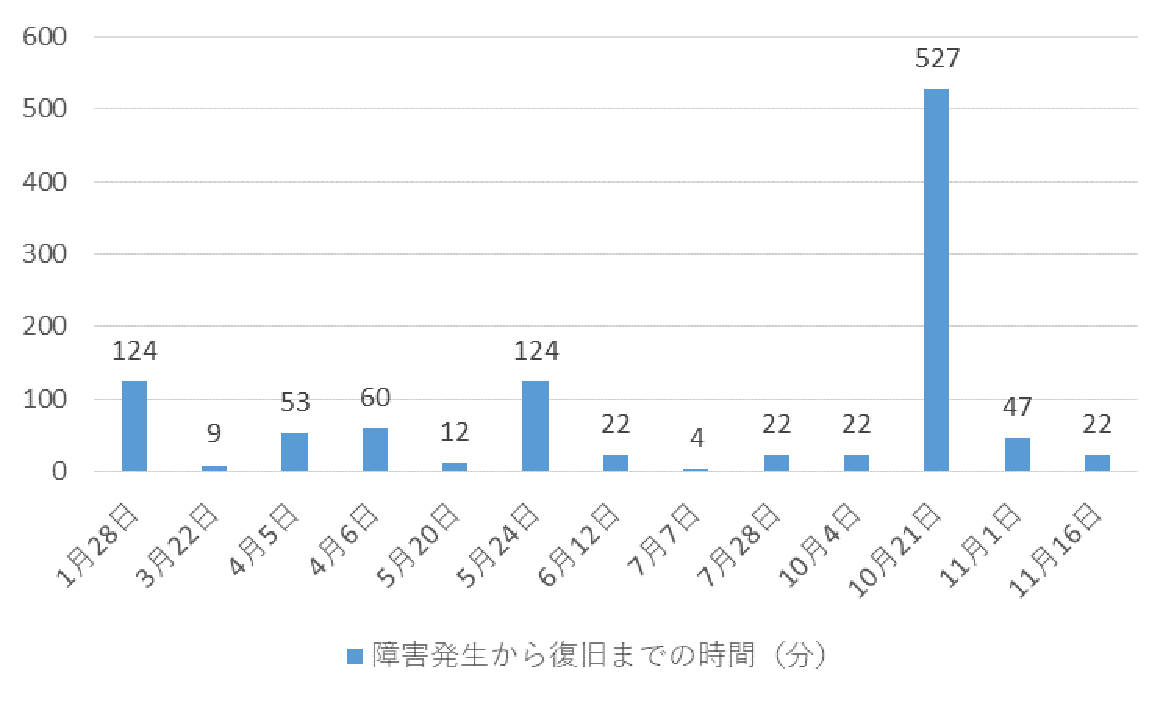
\includegraphics[width=8.5cm,clip]{graph1.pdf}
 \caption{各障害発生時の時間間隔}
 \label{ラベル1}
\end{minipage} &
\begin{minipage}[t]{0.5\hsize}
 \centering
 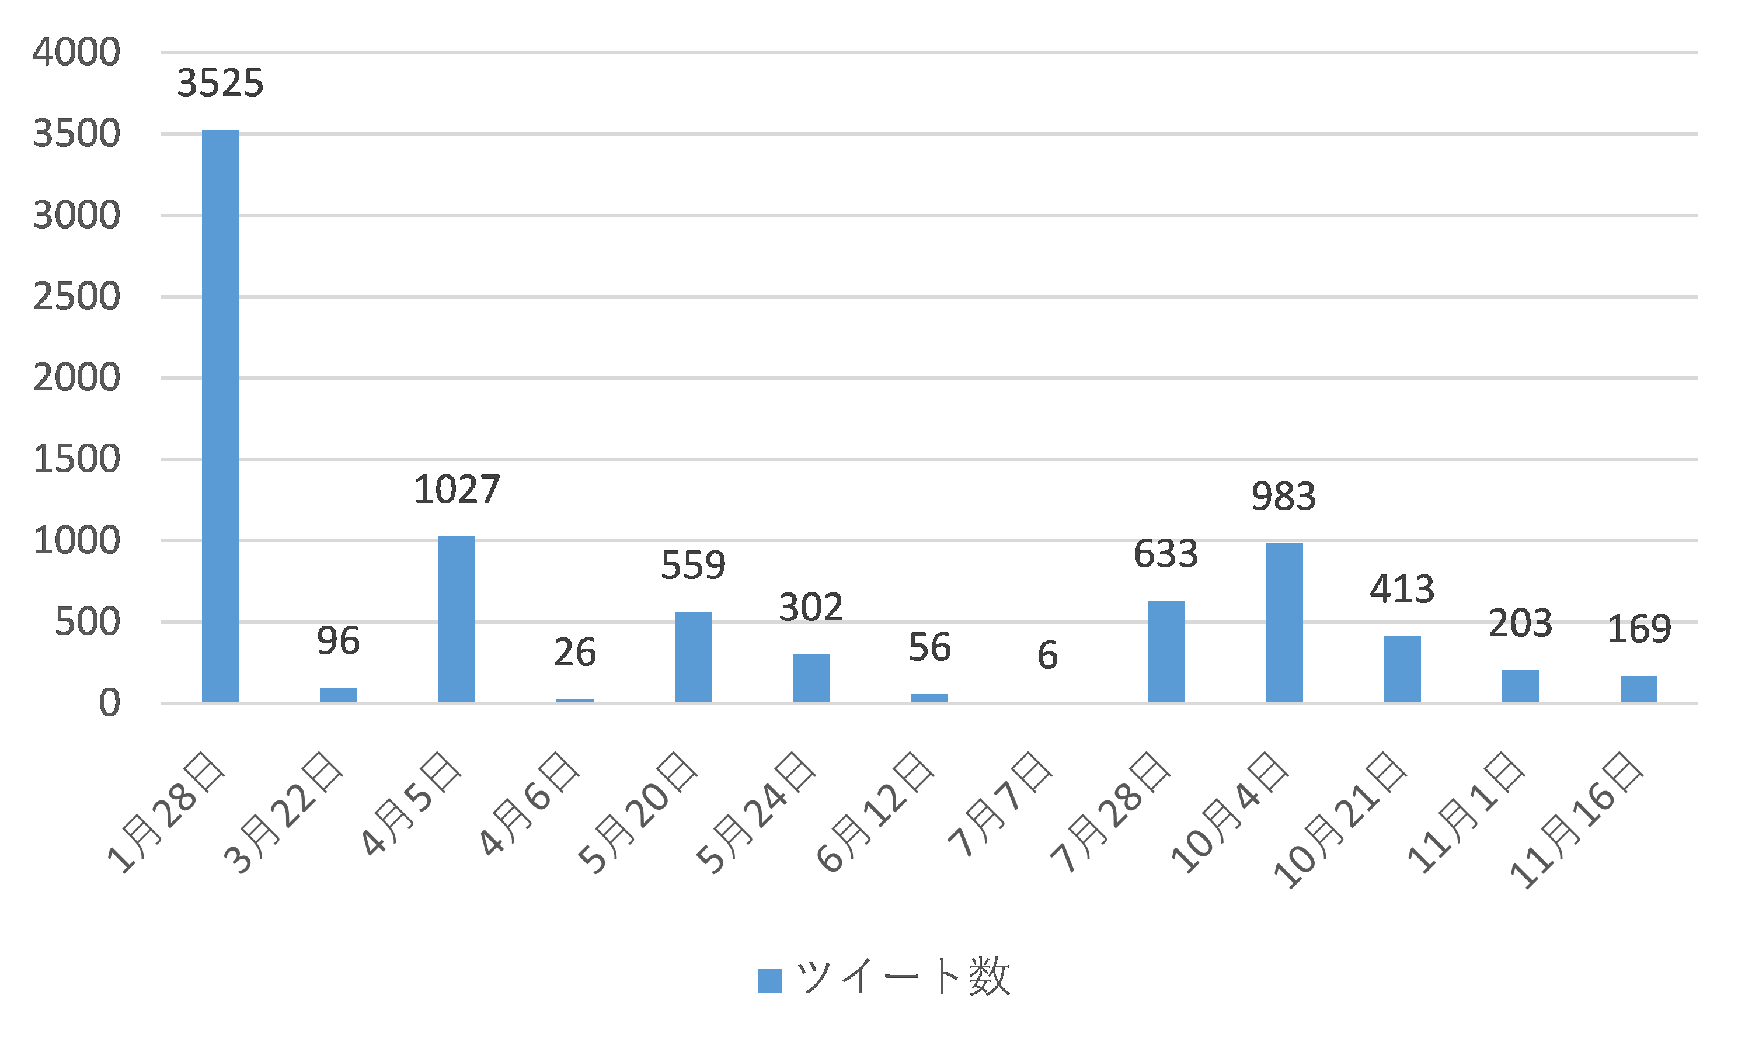
\includegraphics[width=8.5cm,clip]{graph2.pdf}
 \caption{各障害発生時のツイート数}
 \label{ラベル2}
\end{minipage}
\end{tabular}
\end{figure}
\end{center}

13回の障害を見比べてみると,障害発生の曜日,時間帯等によって取得したツイートの数に幅があることが分かった.例えば,日中の約20分間の障害でも祝日と平日では900ツイート以上の差がある.さらに,平日の日中であればツイート数が多いのはもちろんだが,深夜2時台に発生した約10分間の障害でも100件近いツイートが集まった.

また,障害の発生報告と復旧報告が「GitHub Status」よりも平均約7.7分ほど速いということが分かり,Twitterによる情報の速さを実感した.

\section{今後の計画}
以下のように研究を進める計画である.
\begin{enumerate}
 \item 今後は当初予定していなかった時間帯,曜日を加味して分析を行うことも検討する.
 \item 集めたツイート本文のデータから頻出単語を抽出し,多くツイートされている単語を分析する.
 \item 背景で述べた「Slack」「Skype」「Google Drive」の障害発生についても同様の研究を行う.
 \item 4つのWEBサービスのデータの調査した上で,障害発生に対する新しい事前的なリスク対策案を考察する.
\end{enumerate}

\bibliographystyle{junsrt}
\bibliography{biblio}%「biblio.bib」というファイルが必要.

\end{document}
